\ylDisplay{U-toru} % Ülesande nimi
{Tundmatu autor} % Autor
{lahtine} % Voor
{2009} % Aasta
{G 6} % Ülesande nr.
{5} % Raskustase
{
% Teema: Vedelike-mehaanika
\ifStatement
\begin{wrapfigure}[9]{r}{0.4\textwidth}
	\begin{center}
		\vspace{-15pt}
		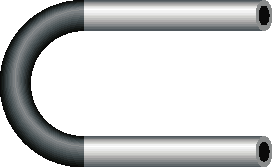
\includegraphics[width=\linewidth]{2009-lahg-06-yl}
	\end{center}
\end{wrapfigure}
Teatud torustikes võib vedeliku surve olla nii tugev, et torud võivad märgatavalt deformeeruda. Vaatleme sellist deformatsiooni U-kujulises torus (vt joonist): kaks sirget pikkusega $l$ terastoru, mille välisraadius on $\sqrt 2$ korda suurem siseraadiusest, on ühendatud sama sisemise raadiusega mittedeformeeruvast materjalist kaarekujulise toruga. Selles U-torus voolab vedelik tihedusega $\rho$ ja konstantse voolukiirusega $v$. Vedeliku hüdrostaatiline rõhk lugeda võrdseks välisrõhuga. U-toru otsad on pinnal jäigalt kinnitatud. Eeldades, et õõnsa terastoru deformatsiooni jaoks toimib Hooke’i seadus, kusjuures jäikustegur avaldub kujul $k = ES/l$ ($E$ on terase nn Young’i konstant, $S$ on toru ristlõike pindala ja $l$ on deformeerimata toru pikkus), leidke toru pikenemine.
\fi


\ifHint
Niisama sirges torus voolav vesi piki-sihilisi deformatsioone ei tekita. Kaarekujulise osa juures, aga survestab vesi väliskülge rohkem kui sisekülge ning tekitab piki-sihilisi pingeid. Pinge täpse suuruse määramiseks on mugav vaadelda kaarekujulist osa tervikuna ning uurida, kuidas vee impulss muutub kaarekujulisse ossa sisenedes ja väljudes.
\fi


\ifSolution
Olgu U-toru siseraadius $r$ ja välisraadius $R = \sqrt 2 r$. Vaatleme eraldi U-toru kaarekujulist osa. Aja $\Delta t$ jooksul siseneb sinna kiirusega $v$ veekogus massiga $\Delta m = \rho \Delta V = \rho \pi r^2vt$, ning samasugune veekogus voolab sealt sama kiirusega välja, seega summaarne vee impulsi muutus aja $\Delta t$ jooksul on $\Delta p= 2\rho\pi r^2v^2 t$, ning jõud, millega vesi mõjub sellele toru osale, on Newtoni teise seaduse põhjal
\[
F=\Delta p/\Delta t= 2\rho\pi r^2v^2. 
\]
Kaarekujuline toru osa on liikumatu, nii et vee poolt rakendatud jõud on tasakaalustatud kahe terastoru elastsusjõuga. Kui terastoru jäikusteguriks võtame $k$, siis on selge, et kehtib võrdus
\[
F = k\Delta l+k\Delta l = 2k\Delta l,
\] 
kus $\Delta l$ on ühe terastoru pikenemine. Teguri $k$ avaldame ülesande tekstis toodud seose kaudu kui $k = ES/l = E\pi \left(R^2 - r^2\right)/l = E\pi r^2/l$ (kogu ristlõike pindalast panustab jäikustegurisse ainult materjaliga kaetud osa) ning seega 
\[
2\rho\pi r^2 v^2= 2E\pi r^2\Delta l/l.
\]
Siit saame ühe toru pikenemiseks $\Delta l=\rho v^2 l/E$ ning kogu U-toru pikenemiseks 
\[
2\Delta l= 2\rho v^2 l/E.
\]
\fi
}